Das Hinzufügen und Löschen eines oder mehreren Artikeln beim App des Kleiderladen ‘Bershka’ ist wie bei vielen anderen Webshops gelöst. 
Es gibt den Warenkorb, bei dem ersichtlich ist welche Artikel ausgewählt wurden, man kann sie löschen oder noch beliebige mehr hinzufügen. 
Allerdings ist meiner Meinung nach, der Prozess des Löschens nicht unbedingt klar. Bin ich im State ‘Warenkorb bearbeiten’ und klicke ‘X’ 
bei dem Produkt, welches ich löschen will, habe ich dann noch die Optionen ‘OK’ und ‘Löschen’. Ich war mir da zuerst nicht sicher, was nun 
gedrückt werden muss und durch Ausprobieren wurde mir dann bewusst, dass wenn man ‘Löschen’ drückt, nur der Bearbeitungsvorgang gelöscht 
wird und nicht das Produkt. Hätte man da anstatt ‘Löschen’ das Wort ‘Abbrechen’ gewählt, wäre dieses Problem nicht aufgetaucht. 

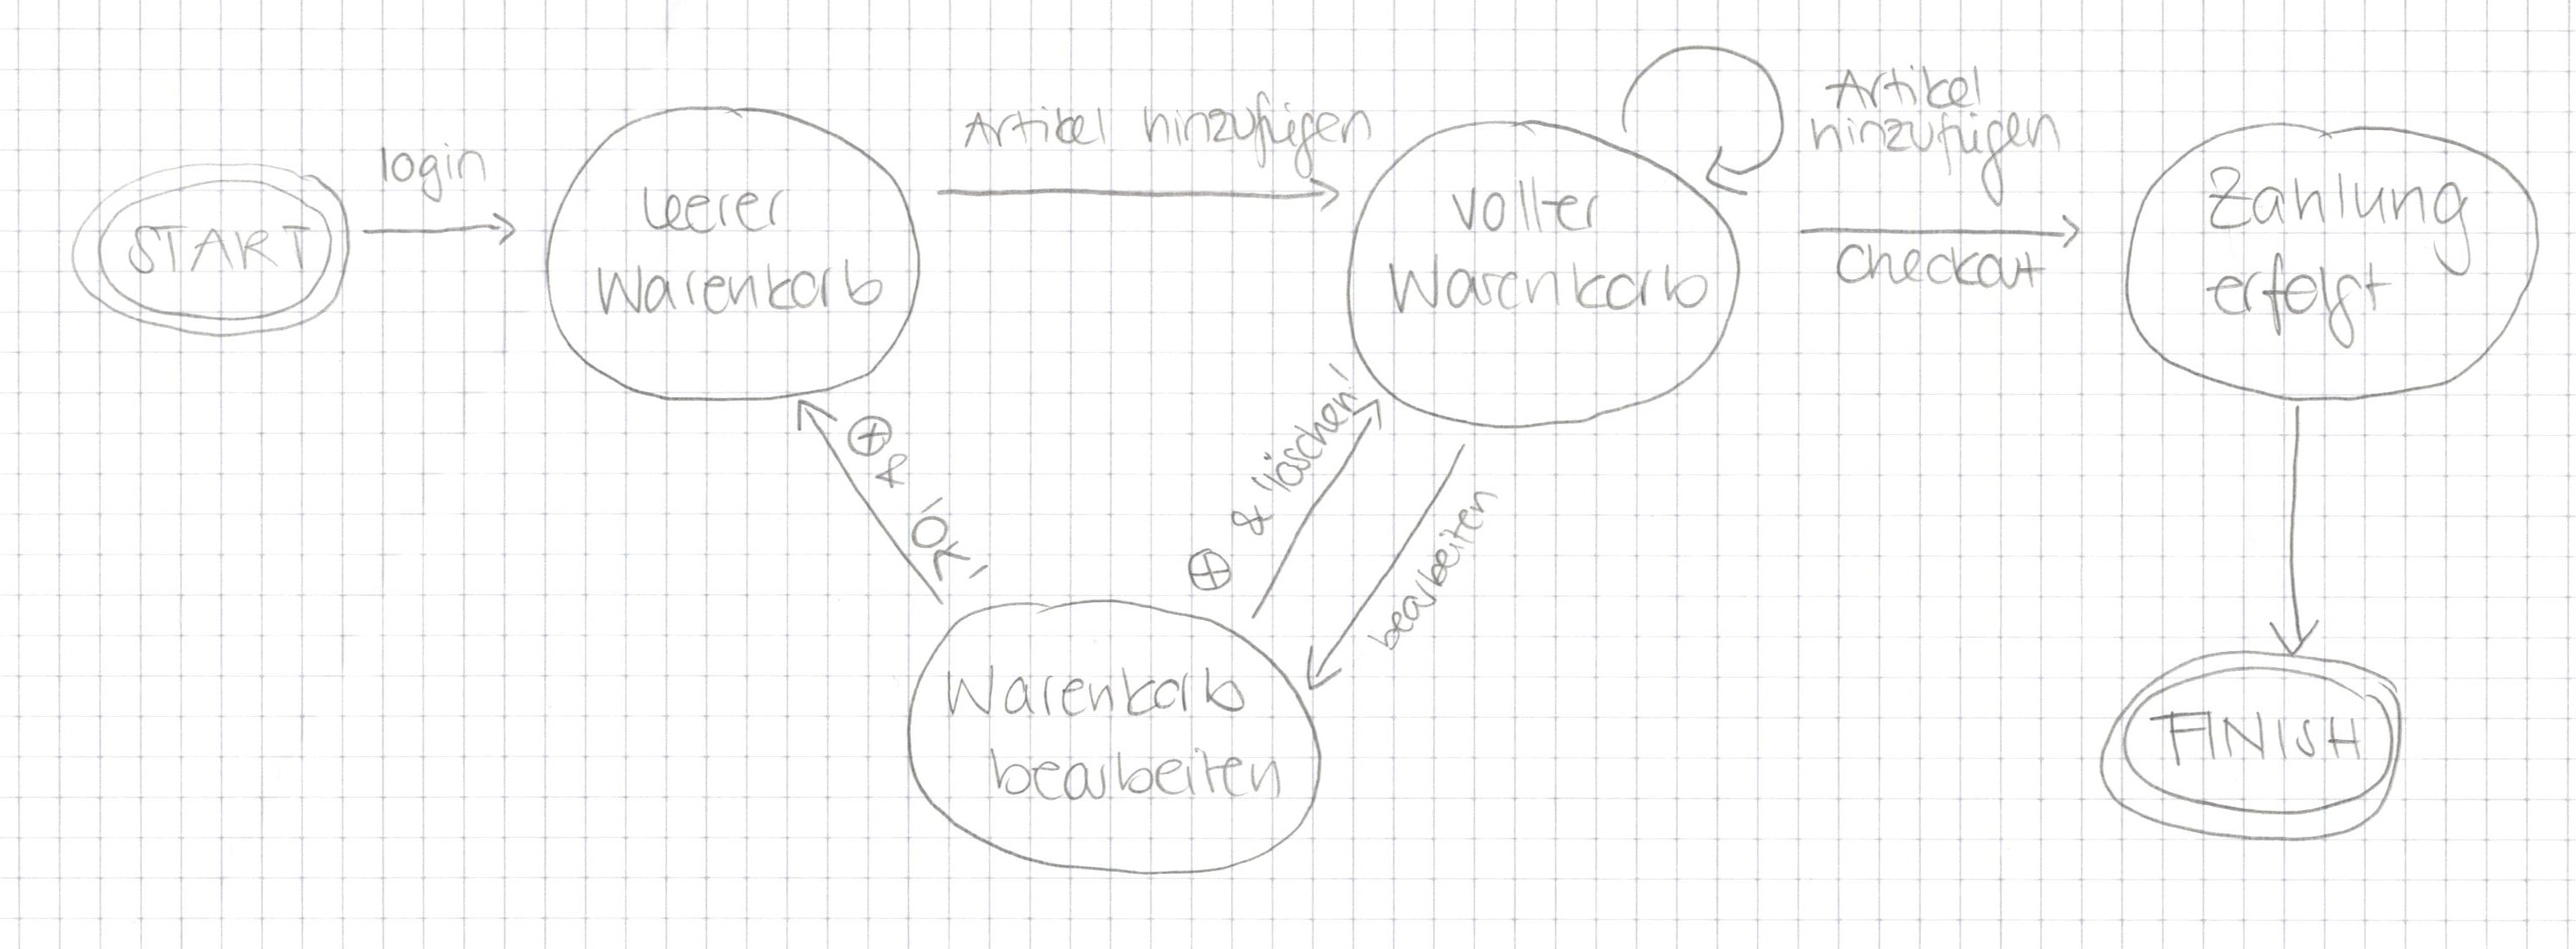
\includegraphics[scale=.5]{images/Scan4_1.jpeg}